\part{Appendix}\label{part:appendices}
\chapter{GOOD Logger}\label{ch:template}

The GOOD Logger is a Python program which can be configured to read from a variety of hardware in the lab and post the data either to the lab's Origin server or a PostgreSQL database. Origin is a program written by Matt Ebert which allows posting to and subscribing to streams or channels of data written to a SQL database. Before the GOOD logger, where GOOD stands for Get Origin Our Data, there were only single-purpose servers in the lab for posting data to origin. The GOOD Logger filled this void by providing a straightforward means to log data from several instruments in the lab in parallel, with a single server that was not embedded in or dependent our experiment control software. 

In its infancy, the GOOD Logger existed in the Hybrid lab, written by Juan Bohorquez to read from some particular instruments. The author of this work, in collaboration with Juan, extended the functionality of the Hybrid logging code to abstract away the details of instrument hardware and reduce the upfront work of the user to entering some parameters in two config files.

Since the publication of \cite{Bohorquez2023}, the GOOD Logger has been adapted by this author to allow writing data to a local database using PostgreSQL\footnote{It has been pointed out by Sam Norrell that without use of Origin, the GOOD Logger becomes the GOD Logger. This name change would be consistent with the notion that the use of Origin was the main limitation of the GOOD Logger.} (shown schematically in Fig. \ref{goodlogger}). This is advantageous in terms of speed when reading from the database, and allows for seamless use with freely available data visualization servers such as Grafana. The ease of this solution stands in contrast to the many attempts at custom plotting solutions there have been in the group in order to cooperate effectively with the Origin server. To-date, the network lab uses the GOOD Logger for monitoring the four Gamma Ion pumps for the two nodes, two open-loop thermocouples in the temperature controlled experiment box (interfaced with a Measurement Computing USB-TEMP device), a Stefan-Meyer 3-axis magnetometer, and various Sinara Zotino channels and coil monitors as needed.

\begin{figure}[!ht]
    \centering
    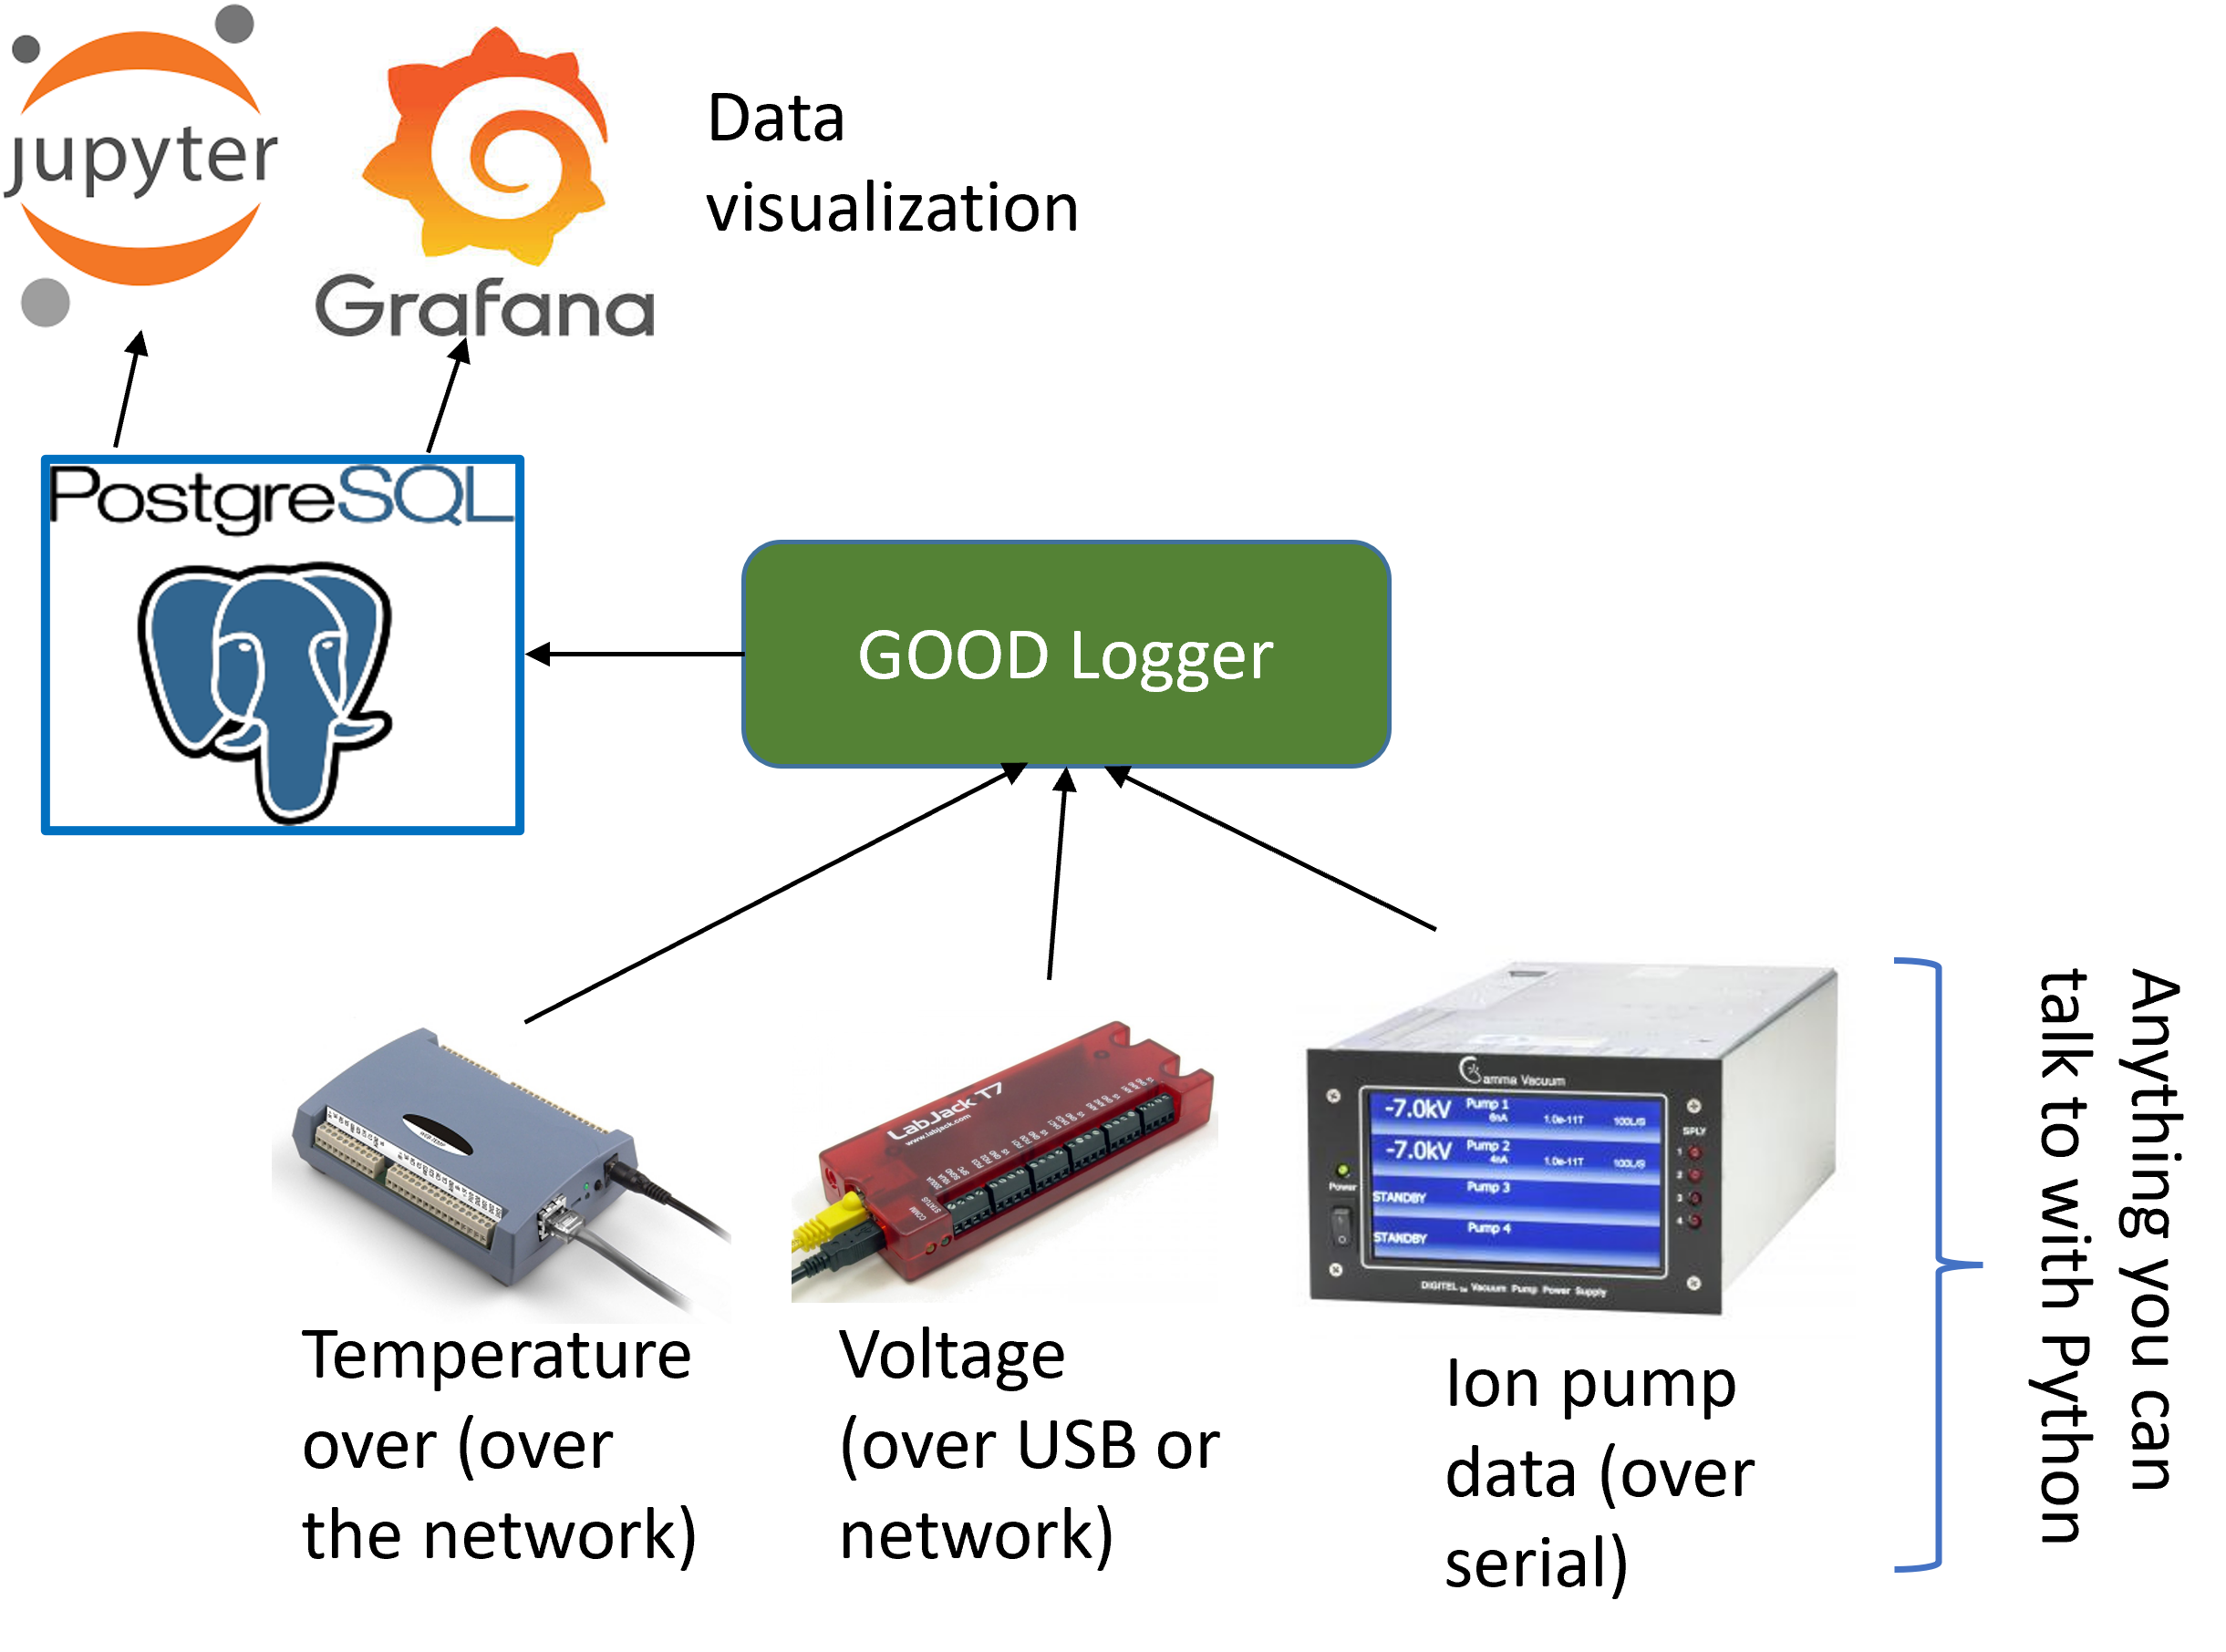
\includegraphics[width=0.5\textwidth]{Images/good_logger_with_postgres.png}
    \caption{Coil driver current monitor outputs, for selected 2D and 3D MOT coils measured with an NI DAQ analog input card and logged using the GOOD Logger. The shaded red region is where experiments are not being run, which shows that abrupt changes occur in the coil values came about without influence by the experimenters.}
    \label{fig:goodlogger}
\end{figure}


The primary motivation for the GOOD Logger arose when transient events in the Rb lab \footnote{This relates to the experiment the author worked on before the existance of network project.} were resulted in sudden loss of the MOT or reduction of atom loading rate during an experiment. The ability to monitor and log signals from multiple sources in a lab asynchronously is of tremendous value for identifying this type of issue. In the case mentioned, we were able to find that some of the homebuilt current drivers for the MOT coils were faulty and exhibited sudden jumps in the current output, shown in Fig. \ref{fig:coiljumps}.

\begin{figure}[!ht]
    \centering
    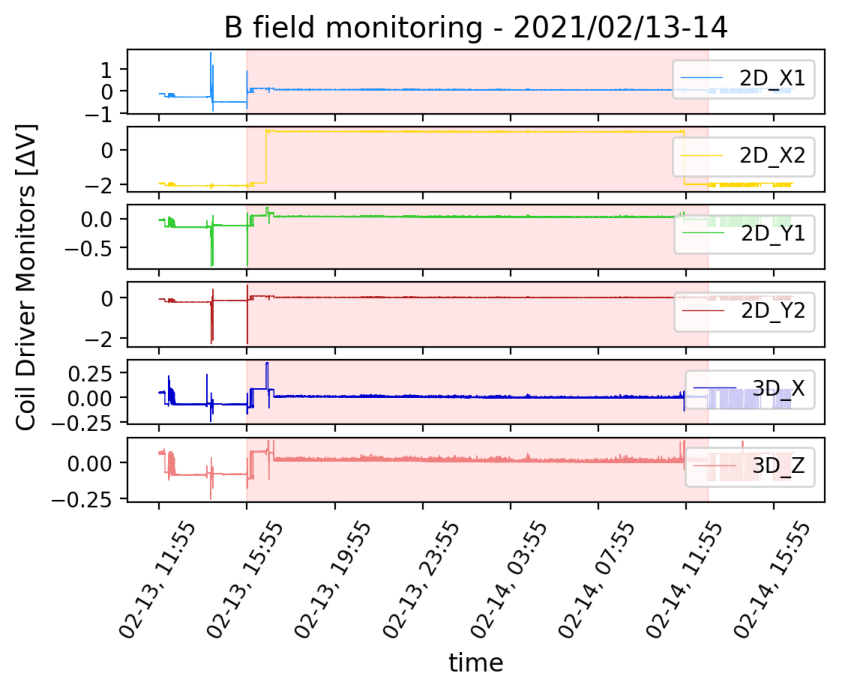
\includegraphics[width=0.9\textwidth]{Images/goodlogger_coil_jumps_20210213_14.pdf}
    \caption{Coil driver current monitor outputs, for selected 2D and 3D MOT coils measured with an NI DAQ analog input card and logged using the GOOD Logger. The shaded red region is where experiments are not being run, which shows that abrupt changes occur in the coil values came about without influence by the experimenters.}
    \label{fig:coiljumps}
\end{figure}



% the hierarchy is 
% chapter,section,subsection,etc
% \end{doublespacing}
